\chapter{Các mặt thế giới, phép quay Wick và tính đối ngẫu giữa các kênh}

\lectureoverview{Một hạt vạch ra một đường thế giới; một dây quét ra một mặt thế giới. Việc lượng tử hóa một trong hai đối tượng đòi hỏi lấy tổng trên các lịch sử, nhưng tổng Lorentz dao động và khó xác định. Biến thời gian của mặt thế giới thành một tọa độ ảo cho ta một lý thuyết Euclid được chi phối bởi phương trình Laplace. Đối xứng bảo giác của nó khi đó biến mặt có khe của một tương tác bốn dây thành một đĩa với bốn điểm chèn trên biên, nơi sự đối xứng giữa kênh trực tiếp và kênh chéo trở nên hiển hiện.}

\section{Từ một đường thế giới đến tổng trên các lịch sử}

Hãy bắt đầu với một hạt tự do. Trong cơ học phi tương đối tính, vị trí của nó là một hàm \(\mathbf x(t)\), và khi đặt khối lượng bằng một, tác dụng của nó là
\begin{equation}
  S_{\mathrm{NR}}[\mathbf x]
  =\frac12\int_{t_1}^{t_2}\dot{\mathbf x}^{\,2}\,dt.
  \label{eq:l07-nr-action}
\end{equation}
Đối với mô tả tương đối tính, tự nhiên hơn là gộp thời gian và không gian vào một vectơ, \(X^\mu(\tau)\), được tham số hóa dọc theo quỹ đạo bởi \(\tau\). Biểu thức bậc hai tương ứng là
\begin{equation}
  S_{\mathrm{rel}}[X]
  =\frac12\int_{\tau_1}^{\tau_2}
  \frac{dX^\mu}{d\tau}\frac{dX_\mu}{d\tau}\,d\tau.
  \label{eq:l07-rel-action}
\end{equation}
Các chỉ số trên và dưới mã hóa sự khác biệt dấu kiểu Lorentz giữa thời gian và không gian.
\editorialnote{Ở đây tác dụng tương đối tính bậc hai được dùng trong một cách tham số hóa đường thế giới cố định. Lựa chọn thay thế hiển nhiên bất biến đối với phép đổi tham số thì tỉ lệ với độ dài riêng, và sẽ được nhắc đến ở phần sau của bài giảng.}

\begin{figure}[H]
  \centering
  \includegraphics[width=0.72\textwidth]{lecture_07_figure_01.png}
  \caption{Tác dụng phi tương đối tính và dạng tương ứng bậc hai tương đối tính của nó được viết cùng nhau trên bảng.}
  \lectureframe{00:03:35}
  \label{fig:l07-particle-actions}
\end{figure}

Về mặt cổ điển, ta cố định hai đầu mút và biến thiên đường đi. Khi đó một hạt tự do đi theo một đường thế giới thẳng với vận tốc không đổi. Cơ học lượng tử đặt ra một câu hỏi khác. Nó không chọn ra một quỹ đạo giữa hai đầu mút; nó hỏi biên độ để hạt bắt đầu ở một điểm và được phát hiện ở điểm kia là bao nhiêu. Mọi đường đi xen giữa đều đóng góp một pha,
\begin{equation}
  K(2,1)=\int_{X(1)}^{X(2)}\!\mathcal D X\,
  e^{iS[X]}.
  \label{eq:l07-feynman-integral}
\end{equation}
Tích phân hàm là một tích phân trên một không gian vô hạn chiều của các đường đi, chứ không phải tích phân thông thường đã xuất hiện bên trong tác dụng.

\begin{figure}[H]
  \centering
  \includegraphics[width=0.72\textwidth]{lecture_07_figure_02.png}
  \caption{Một đường đi tiêu biểu và pha được gán cho nó trước khi lấy tổng trên mọi đường đi.}
  \lectureframe{00:06:21}
  \label{fig:l07-path-integral-board}
\end{figure}

Trong ngôn ngữ tương đối tính, biên độ từ điểm này đến điểm kia là một hàm truyền. Đối với một tương tác, nhiều đoạn đường thế giới gặp nhau. Các tác dụng của chúng được cộng lại, các điểm gặp được lấy tích phân, và ta lấy tổng các giản đồ có những hạt ngoài cần thiết. Vì thế, khai triển quen thuộc theo giản đồ Feynman đã hàm ẩn ngay trong chỉ dẫn lấy tổng trên các lịch sử.

Ở đây, ký hiệu \(S\) sẽ dùng để chỉ tác dụng. Nó không liên quan cả đến entropy lẫn biến Mandelstam \(s\) được dùng gần cuối bài giảng. Việc dùng chung ký hiệu này là do truyền thống hơn là do nó làm sáng tỏ điều gì.

\section{Xoay thời gian sang ngang}

Có một vấn đề nảy sinh ngay với \eqref{eq:l07-feynman-integral}. Mỗi thừa số \(e^{iS}\) đều có độ lớn bằng một. Vì vậy, một quỹ đạo dao động dữ dội và đường thẳng cổ điển đều đi vào với cùng trọng số tuyệt đối; chỉ pha của chúng là khác nhau. Giao thoa triệt tiêu khôi phục hành vi cổ điển, nhưng nó không biến tích phân hình thức ấy thành một đối tượng hội tụ thông thường.

Đưa vào một tham số mới \(s\) theo
\begin{equation}
  \tau=\alpha s,
  \qquad
  d\tau=\alpha\,ds,
  \qquad
  \frac{dX}{d\tau}=\frac{1}{\alpha}\frac{dX}{ds}.
\end{equation}
Khi đó tác dụng bậc hai đổi tỉ lệ thành
\begin{equation}
  \frac12\int d\tau
  \left(\frac{dX}{d\tau}\right)^2
  =
  \frac{1}{2\alpha}\int ds
  \left(\frac{dX}{ds}\right)^2.
  \label{eq:l07-rescaled-action}
\end{equation}
Chọn đường bao tương ứng với \(\alpha=-i\) sẽ biến trọng số dao động thành
\begin{equation}
  e^{iS}
  \longrightarrow
  \exp\!\left[-\frac12\int ds
  \left(\frac{dX}{ds}\right)^2\right]
  =e^{-S_E}.
  \label{eq:l07-euclidean-particle}
\end{equation}

\begin{figure}[H]
  \centering
  \includegraphics[width=0.66\textwidth]{lecture_07_figure_03.png}
  \caption{Trọng số Euclid của hạt sau phép thế thời gian ảo; số mũ là thực và không dương.}
  \lectureframe{00:16:20}
  \label{fig:l07-particle-wick}
\end{figure}

Một đường đi chạy ra rất xa rồi quay lại, hoặc uốn lượn nhanh mà không đi xa, có \(S_E\) dương lớn và bị triệt giảm theo hàm mũ. Kết quả là một tích phân kiểu Wiener, đối với nó tồn tại một lý thuyết hội tụ nghiêm túc. Các đầu mút kế thừa từ \(\tau\) thực nằm trên một đường bao \(s\) ảo. Trong thực hành, người ta tính đối tượng Euclid trong miền hội tụ của nó rồi tiếp tục giải tích kết quả trở lại các biến Lorentz vật lý. Phép toán này là phép quay Wick: thời gian đã được xoay sang bên để phục vụ phép tính, chứ không bị loại bỏ.

\section{Từ các đường thế giới đến các mặt thế giới}

Một hạt điểm có một đường thế giới. Một dây mở quét ra một dải, còn một dây kín quét ra một ống. Các tọa độ \((\sigma,\tau)\) gắn nhãn các điểm trên mặt thế giới hai chiều này, còn
\begin{equation}
  X^\mu=X^\mu(\sigma,\tau)
  \label{eq:l07-embedding}
\end{equation}
cho vị trí không-thời gian của điểm mang nhãn đó. Biết toàn bộ các hàm \(X^\mu\) là xác định đầy đủ lịch sử của dây.

Tác dụng Lorentz bậc hai của mặt thế giới có cùng cấu trúc động năng trừ thế năng như một dây dao động thông thường:
\begin{equation}
  S_{\mathrm{ws}}[X]
  =\frac{T_s}{2}\int d\tau\,d\sigma\,
  \left[
    \partial_\tau X^\mu\partial_\tau X_\mu
    -
    \partial_\sigma X^\mu\partial_\sigma X_\mu
  \right].
  \label{eq:l07-lorentzian-worldsheet}
\end{equation}
Sức căng tổng thể \(T_s\) ấn định thang đo; bài giảng lược bỏ nó để tập trung vào cấu trúc đạo hàm.

\begin{figure}[H]
  \centering
  \includegraphics[width=0.72\textwidth]{lecture_07_figure_04.png}
  \caption{Tác dụng mặt thế giới Lorentz cho
  \(X^\mu(\sigma,\tau)\), với dấu động năng trừ thế năng của nó.}
  \lectureframe{00:24:26}
  \label{fig:l07-worldsheet-action}
\end{figure}

Biên độ của dây được thu được bằng cách mũ hóa tác dụng này và lấy tổng trên mọi mặt nối các cấu hình dây đầu và cuối đã cho:
\begin{equation}
  \mathcal A=\int\mathcal D X\,e^{iS_{\mathrm{ws}}[X]}.
  \label{eq:l07-surface-integral}
\end{equation}
Quy tắc ấy cũng xử lý trường hợp hai dây thành hai, hai thành ba, hoặc bất kỳ cấu hình ngoài nào khác được phép. Các tôpô mặt thế giới khác nhau cũng thuộc vào tổng này. Việc thêm các lỗ là đối tác phía dây của việc thêm các bậc vòng trong khai triển giản đồ hạt điểm.

\begin{figure}[H]
  \centering
  \includegraphics[width=0.66\textwidth]{lecture_07_figure_05.png}
  \caption{Một mặt nối nhiều dây ngoài, với một lỗ biểu diễn một tôpô mặt thế giới khác.}
  \lectureframe{00:27:14}
  \label{fig:l07-surface-topology}
\end{figure}

\begin{classroomqa}
\audiencequestion{Đối với một electron điểm, đạo hàm theo \(\sigma\) có đơn giản là triệt tiêu không? \lecturetimestamp{00:27:56}}
\lecturerresponse{Trước hết, một hạt điểm vốn không có tọa độ \(\sigma\). Tuy vậy, hai bức tranh có liên hệ với nhau: khi các trạng thái ngoài nhẹ so với thang dây và năng lượng của quá trình thấp, các biên độ dây tái tạo các giản đồ Feynman hạt điểm thông thường. Giới hạn đó còn nhiều hơn việc cho một đạo hàm bằng 0.}
\end{classroomqa}

Tích phân trên mặt có cùng vấn đề hội tụ như tích phân đường đi. Sau khi quay Wick thời gian mặt thế giới, dạng Euclid ổn định của nó là
\begin{equation}
  \begin{aligned}
    S_{E,\mathrm{ws}}[X]
    &=\frac{T_s}{2}\int d\tau\,d\sigma\,
      \left[
        \partial_\tau X^\mu\partial_\tau X_\mu
        +\partial_\sigma X^\mu\partial_\sigma X_\mu
      \right],\\
    \mathcal A_E&=\int\mathcal D X\,e^{-S_{E,\mathrm{ws}}}.
  \end{aligned}
  \label{eq:l07-euclidean-worldsheet}
\end{equation}
Giờ đây cả hai đạo hàm đều đi vào với cùng dấu dương. Một mặt dao động dữ dội hoặc bị kéo căng mạnh có tác dụng Euclid lớn và bị triệt giảm.

\begin{figure}[H]
  \centering
  \includegraphics[width=0.72\textwidth]{lecture_07_figure_06.png}
  \caption{Mật độ mặt thế giới Euclid dương sau khi
  \(\tau\) được quay sang thời gian ảo.}
  \lectureframe{00:34:29}
  \label{fig:l07-worldsheet-wick}
\end{figure}

Cũng có một cách phát biểu trực tiếp về mặt hình học. Có thể gán cho một hạt tương đối tính một tác dụng tỉ lệ với độ dài riêng của quỹ đạo nó; có thể gán cho một dây một tác dụng tỉ lệ với diện tích không-thời gian của mặt thế giới của nó. Dạng sau là tác dụng Nambu--Goto. Dạng mặt thế giới bậc hai được dùng ở đây theo quy ước được gọi là dạng Polyakov và dễ hơn nhiều cho phép tính hiện tại.
\editorialnote{Bài giảng có kèm một trao đổi hài hước về cách đặt tên trong lịch sử và cũng nhắc đến tác dụng Liouville liên quan cùng các điều kiện biên Dirichlet. Việc suy dẫn không cần đến bất kỳ khẳng định ưu tiên nào: chỉ dùng sự tương đương giữa mô tả theo diện tích và mô tả với metric phụ trợ.}

\section{Phương trình chuyển động Euclid}

Các tọa độ \(\sigma\) và \(\tau\) chỉ là các nhãn trên mặt. Vì vậy câu hỏi tiếp theo là không thể tránh khỏi: những phép gắn nhãn lại nào để nguyên lý thuyết? Câu trả lời dễ thấy nhất từ phương trình chuyển động. Biến phân \eqref{eq:l07-euclidean-worldsheet} cho, theo từng thành phần,
\begin{equation}
  \partial_\tau^2X^\mu+\partial_\sigma^2X^\mu=0.
  \label{eq:l07-laplace}
\end{equation}
Trước phép quay Wick, dấu tương đối là âm và đây là một phương trình sóng. Trong chữ ký Euclid, cả hai dấu đều dương, nên đây là phương trình Laplace hai chiều.

\begin{classroomqa}
\audiencequestion{Đây có phải là phương trình của một màng trống dao động không?
\lecturetimestamp{00:41:50}}
\lecturerresponse{Nó có liên hệ rất gần, nhưng một màng trống dao động còn có một tọa độ thời gian thực và vì thế tuân theo một phương trình sóng. Phương trình ở đây là phương trình Laplace Euclid. Thế điện tĩnh trong một miền không có điện tích cho một ví dụ quen thuộc trực tiếp hơn.}
\end{classroomqa}

\begin{classroomqa}
\audiencequestion{Tác dụng chứa các đạo hàm bậc nhất. Vì sao phương trình của nó lại chứa các đạo hàm bậc hai? \lecturetimestamp{00:42:44}}
\lecturerresponse{Biến phân một hạng tử bậc hai theo đạo hàm bậc nhất rồi lấy tích phân từng phần sẽ chuyển một đạo hàm lên đạo hàm bậc nhất ấy. Đây là phiên bản của lý thuyết trường trong đó \(\dot x^{\,2}\) ở trong tác dụng sinh ra \(\ddot x\) trong phương trình chuyển động.}
\end{classroomqa}

\begin{figure}[H]
  \centering
  \includegraphics[width=0.68\textwidth]{lecture_07_figure_07.png}
  \caption{Phương trình Laplace với dấu cộng và dòng rời rạc đầu tiên được dùng để diễn giải các đạo hàm bậc hai của nó.}
  \lectureframe{00:43:30}
  \label{fig:l07-laplace-board}
\end{figure}

Để thấy hình học, trước hết hãy rời rạc hóa một tọa độ với khoảng cách \(\epsilon\). Đạo hàm bậc nhất là hiệu giữa các điểm lân cận, còn đạo hàm bậc hai là hiệu của các hiệu lân cận:
\begin{equation}
  \frac{d^2X}{ds^2}\bigg|_{2}
  \longrightarrow
  \frac{X(3)-2X(2)+X(1)}{\epsilon^2}.
  \label{eq:l07-second-difference}
\end{equation}

\begin{figure}[H]
  \centering
  \includegraphics[width=0.72\textwidth]{lecture_07_figure_08.png}
  \caption{Đường thẳng được đánh số, một mảnh lưới nhỏ và khai triển sai phân hữu hạn của một đạo hàm bậc hai.}
  \lectureframe{00:45:51}
  \label{fig:l07-finite-difference-board}
\end{figure}

Bây giờ hãy rời rạc hóa mặt phẳng \((\sigma,\tau)\). Gắn nhãn bốn điểm lân cận gần nhất của điểm trung tâm \(5\) là \(1,2,3,4\). Phương trình \eqref{eq:l07-laplace} trở thành
\begin{equation}
  X(1)+X(2)+X(3)+X(4)-4X(5)=0,
\end{equation}
hay
\begin{equation}
  X(5)=\frac14\bigl[X(1)+X(2)+X(3)+X(4)\bigr].
  \label{eq:l07-mean-value}
\end{equation}

\begin{figure}[H]
  \centering
  \includegraphics[width=0.72\textwidth]{lecture_07_figure_09.png}
  \caption{Phương trình sai phân hữu hạn hai chiều hoàn chỉnh: giá trị ở tâm bằng trung bình của bốn điểm lân cận của nó.}
  \lectureframe{00:48:26}
  \label{fig:l07-mean-value-board}
\end{figure}

Tính chất giá trị trung bình này đúng cho một hình vuông vi phân ở mọi định hướng. Đó là nội dung hình học địa phương của phương trình Laplace và là chiếc cầu nối tới đối xứng bảo giác.

\section{Tọa độ bảo giác}

Xét một phép đổi từ \((\sigma,\tau)\) sang
\((\sigma',\tau')\). Một biến dạng tổng quát biến một hình vuông nhỏ thành một tứ giác tùy ý. Những phép biến đổi đặc biệt có liên quan ở đây biến mọi hình vuông vi phân thành một hình vuông vi phân khác, có thể bị quay và đổi tỉ lệ. Tương đương, chúng bảo toàn các góc mà tại đó các đường cong gặp nhau. Đó là các phép biến đổi bảo giác.

\begin{figure}[H]
  \centering
  \includegraphics[width=0.68\textwidth]{lecture_07_figure_10.png}
  \caption{Một hình vuông địa phương được ánh xạ sang một hình nhỏ khác, đồng thời kiểm tra xem các góc của nó có được bảo toàn theo nghĩa bảo giác hay không.}
  \lectureframe{00:53:25}
  \label{fig:l07-conformal-board}
\end{figure}

\begin{classroomqa}
\audiencequestion{Nếu các góc được bảo toàn, về cơ bản phép biến đổi có phải chỉ là một phép quay không? \lecturetimestamp{00:53:31}}
\lecturerresponse{Chỉ theo nghĩa địa phương, và ngay cả khi đó một phép đổi thang chung cũng được cho phép. Góc quay địa phương và hệ số tỉ lệ có thể thay đổi từ điểm này sang điểm khác, vì thế lưới tọa độ có thể uốn cong, nở ra ở vùng này và co lại ở vùng khác mà vẫn bảo toàn hình dạng vi phân.}
\end{classroomqa}

Một ánh xạ bảo toàn góc không nhất thiết bảo toàn kích thước. Nếu kích thước cũng được giữ cố định ở mọi nơi, các khả năng sẽ thu hẹp lại thành lớp cứng nhỏ hơn rất nhiều gồm các phép tịnh tiến và quay. Thay vào đó, các ánh xạ bảo giác bảo toàn hình dạng địa phương. Vì thế một phép chiếu bản đồ có thể giữ nguyên hình dạng của một hòn đảo nhỏ đồng thời làm méo rất mạnh diện tích của nó.

\begin{classroomqa}
\audiencequestion{Một ánh xạ bảo giác có tương đương với việc nói rằng hệ tọa độ là phẳng không? \lecturetimestamp{00:55:35}}
\lecturerresponse{Không. Tính phẳng và tính bảo giác là hai mệnh đề khác nhau. Một ánh xạ bảo giác có thể dùng các đường tọa độ cong; điều nó bảo toàn là góc giữa các đường cong cắt nhau. Phép chiếu bản đồ kiểu Mercator là một ví dụ quen thuộc về việc bảo toàn hình dạng địa phương đi kèm với biến dạng thang đo đáng kể.}
\end{classroomqa}

Trong hai chiều, các phép biến đổi cần thiết được sinh ra một cách địa phương bởi các hàm giải tích của một tọa độ phức
\begin{equation}
  z=\sigma+i\tau.
\end{equation}
Các biên hữu hạn có thể thay đổi hình dạng bề ngoài một cách rất mạnh. Một miền hình vuông có thể được ánh xạ thành một miền trơn, trong đó các góc ban đầu được đưa tới những điểm bình thường trên biên mới chứ không phải tới các điểm nổi bật về mặt thị giác của nó. Không có mâu thuẫn nào cả: tính bảo giác là một điều kiện địa phương ở bên trong, và ánh xạ bảo toàn các góc vi phân ở mọi nơi mà nó là chính quy.

\begin{classroomqa}
\audiencequestion{Có phải chính tự do chọn tọa độ này là lý do sơ đồ nối--tách trước đó có thể được chọn đối xứng không?
\lecturetimestamp{00:56:32}}
\lecturerresponse{Đúng. Cùng tự do bảo giác bảo toàn các phương trình trên mặt thế giới cho phép ta thay dải tương tác vụng về bằng một miền đối xứng hơn. Tự do còn lại không loại bỏ tham số nối--tách vật lý; nó đóng gói lại tham số ấy thành vị trí tương đối của các điểm chèn trên biên.}
\end{classroomqa}

\section{Mặt có khe và đĩa}

Quay lại tán xạ bốn dây. Hai dây hở đi vào, các đầu mút của chúng nối lại với nhau, dây kết hợp truyền đi, rồi sau đó tách ra. Khi được vẽ như một mặt thế giới phẳng, quá trình này là một dải vô hạn bị rạch một khe từ mỗi đầu. Khoảng cách \(\tau_0\) giữa các đỉnh của những khe ấy là thời gian sống của dây trung gian, và biên độ được tích phân theo đại lượng đó.

\begin{figure}[H]
  \centering
  \includegraphics[width=0.72\textwidth]{lecture_07_figure_11.png}
  \caption{Dải có hai khe biểu diễn hai dây hở nối lại với nhau, cùng truyền đi, rồi lại tách ra.}
  \lectureframe{01:00:20}
  \label{fig:l07-slit-strip}
\end{figure}

Sau khi Euclid hóa, các trường nhúng trên miền này thỏa mãn phương trình Laplace. Vì vậy, tính bất biến bảo giác cho phép ánh xạ dải có khe thành một đĩa. Một cách để thấy tôpô là phân lá đĩa bằng các đường tròn đồng tâm rồi biến dạng liên tục các đường cong khép kín ấy cho đến khi chúng lấp đầy miền có khe. Các đầu ở vô cực trở thành những điểm biên đặc biệt dưới ánh xạ này.

\begin{figure}[H]
  \centering
  \includegraphics[width=0.72\textwidth]{lecture_07_figure_12.png}
  \medskip

  \begin{adjustbox}{max width=\linewidth}
  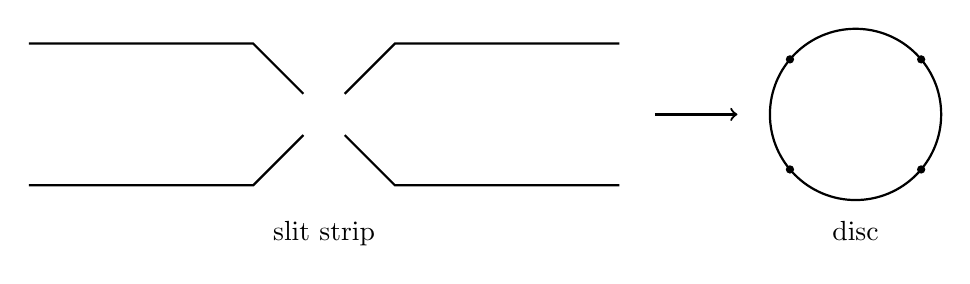
\begin{tikzpicture}[x=0.75cm,y=0.75cm]
    \draw[thick] (-5,1.2) -- (-1.2,1.2) -- (-0.35,0.35);
    \draw[thick] (-5,-1.2) -- (-1.2,-1.2) -- (-0.35,-0.35);
    \draw[thick] (0.35,0.35) -- (1.2,1.2) -- (5,1.2);
    \draw[thick] (0.35,-0.35) -- (1.2,-1.2) -- (5,-1.2);
    \draw[->,thick] (5.6,0) -- (7.0,0);
    \draw[thick] (9.0,0) circle (1.45);
    \foreach \a in {40,140,220,320} \fill (9.0,0) ++(\a:1.45) circle (1.5pt);
    \node[below] at (0,-1.65) {slit strip};
    \node[below] at (9.0,-1.65) {disc};
  \end{tikzpicture}
  \end{adjustbox}
  \caption{Phép so sánh các đường mức trên bảng và một sơ đồ rõ ràng của ánh xạ bảo giác từ dải có khe lên một đĩa. Bốn đầu ngoài trở thành bốn điểm biên đặc biệt.}
  \lectureframe{01:04:46}
  \label{fig:l07-strip-to-disc}
\end{figure}

Các trạng thái ngoài không bị mất đi trong sự thay đổi tọa độ này. Xung lượng, loại hạt và mức dao động phải được chèn vào bốn điểm đặc biệt ấy. Các đối tượng hình thức mang thông tin đó là các toán tử đỉnh. Việc xây dựng chi tiết của chúng được để lại cho phần sau, nhưng vai trò của chúng đã rõ: chúng biến một tích phân đường trên mặt thế giới vốn đồng nhất thành một thí nghiệm tán xạ xác định.

Sau khi dùng các phép biến đổi bảo giác của đĩa để đưa ba điểm biên tới những vị trí tham chiếu thuận tiện, vẫn còn lại một vị trí tương đối thực. Nó có thể được biểu diễn bằng tỷ số kép của bốn điểm biên có thứ tự. Đây là phiên bản trên đĩa của thời gian sống \(\tau_0\) trước đây.

\begin{figure}[H]
  \centering
  \includegraphics[width=0.62\textwidth]{lecture_07_figure_13.png}
  \caption{Bốn điểm chèn trên biên của đĩa. Tự do bảo giác loại bỏ tất cả ngoại trừ một môđun thực của cấu hình có thứ tự của chúng.}
  \lectureframe{01:10:55}
  \label{fig:l07-four-points}
\end{figure}

Vì thế, tích phân theo thời gian sống không hề biến mất. Nó đã trở thành một tích phân theo môđun còn lại ấy. Với một tọa độ quy ước \(0<z<1\), tích phân bốn điểm của dây hở có cùng dạng như đã gặp trong bài giảng trước,
\begin{equation}
  \mathcal A(s,t)\propto
  \int_0^1 z^{-s-1}(1-z)^{-t-1}\,dz.
  \label{eq:l07-modulus-integral}
\end{equation}

\section{Hai giới hạn của cùng một mặt}

Ở một đầu của không gian môđun, hai điểm chèn gắn với cặp đi vào tiến lại gần nhau. Trong tọa độ dải có khe, điều này là một khoảng dài giữa lúc nối và lúc tách: một dây trung gian ở kênh trực tiếp truyền trong thời gian dài. Ở đầu kia, một cặp kề nhau khác tiến lại gần nhau. Khi đó cùng một mặt ấy tự nhiên được hiểu như một sự trao đổi ở kênh chéo. Trên dải, các mô tả này trông như không liên quan, nhưng chúng là hai giới hạn biên kề nhau của cùng một tích phân trên đĩa.

Quay lại quy ước mostly-plus của bài giảng trước,
\begin{equation}
  -s=(k_1+k_2)^2,
  \qquad
  -t=(k_1+k_3)^2.
  \label{eq:l07-mandelstam}
\end{equation}
Giới hạn trực tiếp sắp xếp các cực theo \(s\); giới hạn chéo sắp xếp các cực theo \(t\).
\editorialnote{Gần cuối bài giảng, bảng dùng một ký hiệu dấu viết tắt cho các bất biến Mandelstam, đồng thời cũng đồng nhất \(s\) với bình phương dương của năng lượng trong hệ khối tâm. Phương trình \eqref{eq:l07-mandelstam} giữ nguyên quy ước mostly-plus đã được thiết lập ở Bài giảng 6.}

\begin{figure}[H]
  \centering
  \includegraphics[width=0.62\textwidth]{lecture_07_figure_14.png}
  \caption{Hai sơ đồ kênh: sự truyền dài theo một định hướng và sự trao đổi theo định hướng chéo.}
  \lectureframe{01:19:27}
  \label{fig:l07-channel-diagrams}
\end{figure}

\begin{figure}[H]
  \centering
  \includegraphics[width=0.72\textwidth]{lecture_07_figure_15.png}
  \caption{Bảng quay lại các ghép cặp xung lượng của kênh \(s\) và kênh \(t\) khi so sánh hai giới hạn của môđun đĩa.}
  \lectureframe{01:19:40}
  \label{fig:l07-st-board}
\end{figure}

Một đối tượng giải tích vì thế cung cấp cả hai khai triển:
\begin{equation}
  \mathcal A(s,t)=\mathcal A(t,s).
\end{equation}
Đây là đối ngẫu kênh. Trong ngôn ngữ cộng hưởng ban đầu, việc một tổng trên các trạng thái của kênh trực tiếp đồng thời cũng có thể mã hóa sự trao đổi ở kênh chéo có vẻ thật kỳ diệu. Trên mặt thế giới Euclid, đối xứng bảo giác giải thích vì sao hai mô tả ấy thuộc cùng một mặt. Về mặt lịch sử, cách diễn giải này xuất hiện rất nhanh sau khi biên độ Veneziano được phát hiện vào 1969.

\begin{classroomqa}
\audiencequestion{Có mô tả dải có khe nào tương ứng với định hướng chéo không? \lecturetimestamp{01:20:49}}
\lecturerresponse{Có, nhưng hướng được gọi là thời gian phải được chọn khác đi. Cùng một mặt thế giới Euclid ấy có thể được cắt lát sao cho một cặp đầu ngoài khác nằm ở quá khứ xa và tương lai xa. Chính cách cắt lát thay thế đó là lý do một mặt thế giới duy nhất cho phép hơn một cách diễn giải theo kênh.}
\end{classroomqa}

\begin{classroomqa}
\audiencequestion{Thời gian mà các dây còn nối với nhau có được quyết định bởi hằng số ghép không? \lecturetimestamp{01:21:39}}
\lecturerresponse{Không có thời gian sống cố định nào được chọn. Thời gian sống là một biến tích phân và mọi giá trị đều đóng góp. Hằng số ghép điều khiển trọng số cho sự nối và tách---tương đương, cường độ phân rã---và đi vào biên độ dưới dạng một thừa số nhân; nó không thay thế tích phân theo môđun.}
\end{classroomqa}